\documentclass[12pt,a4paper]{book}
\usepackage[utf8]{inputenc}
\usepackage[spanish]{babel}
\addto\captionsspanish{\renewcommand{\contentsname}{Índice general}}
\usepackage{amsmath}
\usepackage{amsfonts}
\usepackage{indentfirst}
\usepackage{amssymb}
\usepackage{graphicx}
\usepackage{multirow}
\usepackage{multicol}
\usepackage[left=2.54cm,right=2.54cm,top=1.3cm,bottom=4.2cm,headsep=30pt,footskip=0.02cm]{geometry}
\usepackage{setspace}
\usepackage{titlesec}
\usepackage{fancyhdr}
\usepackage{enumitem}
\usepackage{longtable}
% \usepackage{tocbibind} % Evita que el índice agregue entradas extra (Índice/Bibliografía)
\usepackage{pgfgantt}
\usepackage{pdflscape}
\usepackage{tocloft}
\usepackage{listings}
\usepackage{xcolor}
\usepackage{array}
\usepackage[table]{xcolor}
\usepackage{adjustbox}
\usepackage{newtxtext}
\usepackage{newtxmath}
\usepackage{media9}
\usepackage{float}
\usepackage{caption}
\usepackage[table,xcdraw]{xcolor}
\usepackage{tabularx}
\usepackage{hyperref}
\usepackage{csquotes}
\usepackage[numbers,sort&compress]{natbib}
\bibliographystyle{plainnat}

% Configuración de titlesec
\titleformat{\section}{\Large\bfseries}{\thesection}{1em}{}
\titleformat{\subsection}{\large\bfseries}{\thesubsection}{1em}{}
\titleformat{\subsubsection}{\normalsize\bfseries}{\thesubsubsection}{1em}{}

\titlespacing*{\section}{0pt}{18pt}{12pt}
\titlespacing*{\subsection}{0pt}{14pt}{8pt}
\titlespacing*{\subsubsection}{0pt}{12pt}{6pt}
\setlength{\parindent}{1.27cm}

\lstset{
    inputencoding=utf8,
    extendedchars=true,
    literate=%
        {á}{{\'a}}1 {é}{{\'e}}1 {í}{{\'i}}1 {ó}{{\'o}}1 {ú}{{\'u}}1
        {Á}{{\'A}}1 {É}{{\'E}}1 {Í}{{\'I}}1 {Ó}{{\'O}}1 {Ú}{{\'U}}1
        {ñ}{{\~n}}1 {Ñ}{{\~N}}1
}

% Configuración de encabezados y pies de página
\pagestyle{fancy}
\fancyhf{}
\fancyfoot[R]{\raisebox{-10pt}{\thepage}}
% \setlength{\headheight}{70pt}
% \fancyhead[L]{\makebox[0pt]{\includegraphics[height=1.7cm]{imagenes/escudo-1-1.png}}}
% \fancyhead[R]{\makebox[0pt]{\includegraphics[height=1.7cm]{imagenes/logoCarrera.png}}}
% \fancyhead[C]{
%     \footnotesize
%     \small{Inteligencia Artificial            \hspace{6cm}        26-I} \\
%     \vspace{0.1cm}
% }
\fancyfoot[R]{\thepage}
\setlength{\headheight}{3cm}
\setlength{\headsep}{0.5cm}
\renewcommand{\headrulewidth}{0pt}
\renewcommand{\footrulewidth}{0pt}

\fancypagestyle{plain}{
    \fancyhf{}
    \fancyfoot[R]{\raisebox{5pt}{\thepage}}
    \renewcommand{\headrulewidth}{0pt}
}

% Configuración de captions
\captionsetup[table]{
    labelfont=bf,
    textfont=it,
    labelsep=colon
}
\captionsetup[figure]{
    labelfont=bf,
    textfont=it,
    labelsep=colon
}

\definecolor{codebg}{rgb}{0.95,0.95,0.92}
\definecolor{keywordcolor}{rgb}{0.0,0.0,0.8}
\definecolor{commentcolor}{rgb}{0.0,0.5,0.0}
\definecolor{stringcolor}{rgb}{0.58,0.0,0.82}
\definecolor{numbercolor}{rgb}{0.5,0.5,0.5}

\lstset{
    language=Python,
    backgroundcolor=\color{codebg},
    basicstyle=\ttfamily\small,
    keywordstyle=\color{keywordcolor}\bfseries,
    commentstyle=\color{commentcolor}\itshape,
    stringstyle=\color{stringcolor},
    numberstyle=\tiny\color{numbercolor},
    numbers=left,
    stepnumber=1,
    numbersep=5pt,
    showstringspaces=false,
    breaklines=true,
    frame=single,
    tabsize=2
}

\lstset{
  language=C++,
  basicstyle=\ttfamily\footnotesize,
  keywordstyle=\color{blue}\bfseries,
  stringstyle=\color{orange},
  commentstyle=\color{gray}\itshape,
  numbers=left,
  numberstyle=\tiny\color{gray},
  stepnumber=1,
  numbersep=10pt,
  frame=single,
  rulecolor=\color{black},
  backgroundcolor=\color{black!2},
  tabsize=2,
  captionpos=b,
  breaklines=true,
  showstringspaces=false
}

\lstset{
    language=SQL,
    basicstyle=\small\ttfamily,
    numbers=left,
    numberstyle=\tiny,
    numbersep=5pt,
    frame=none,
    breaklines=true,
    breakatwhitespace=true,
    showstringspaces=false,
    tabsize=2,
    commentstyle=\color{green!50!black},
    keywordstyle=\color{blue},
    stringstyle=\color{red},
    captionpos=b
}

\setlength{\parindent}{0pt}
\setlength{\parskip}{0.5em}

\begin{document}

\begin{titlepage}
 \thispagestyle{empty}
 \doublespacing
    \begin{center}
        {\large UNIVERSIDAD NACIONAL DE SAN ANTONIO ABAD DEL CUSCO} \\[0.1cm]
        {\large FACULTAD DE INGENIERÍA ELÉCTRICA, ELECTRÓNICA, INFORMÁTICA Y MECÁNICA} \\[0.1cm]
        {\large ESCUELA PROFESIONAL DE INGENIERÍA INFORMÁTICA Y DE SISTEMAS} \\[0.5cm]
    \begin{figure}[htb]
    \centering
    
\includegraphics[scale=0.6]{figures/UNSAAC.png}
    \end{figure}
        
        {\large \textbf{Trabajo}} \\
        \rule{140mm}{0.7mm} \\
        {\Large \textbf{''Sistema de cableado estructurado del E.P de Enfermeria''}} \\
        \rule{140mm}{0.7mm} \\[0.6cm]
        
        \begin{tabular}{@{} l l @{}}
            \textbf{\fontsize{14}{14}\selectfont Asignatura:} & Redes I \\[0.1cm]
            \textbf{\fontsize{14}{14}\selectfont Docente:}    & Ing. Dueñas Bustinza Darío Francisco \\[0.1cm]
            \textbf{\fontsize{14}{14}\selectfont Integrantes:} & - integrante 1 \\[0.07cm] 
                                                               & - Mamani Flores Natan \\[0.07cm]
                                                               & - Integrante 3 \\[0.07cm]
                                                               & - Integrante 4 \\[0.07cm]
            
            \textbf{\fontsize{14}{14}\selectfont Semestre:}   & 2026-I \\
        \end{tabular} \\[0.7cm]
        
        \textbf{\fontsize{15}{14}\selectfont Cusco-Perú} \\
        \textbf{\fontsize{15}{14}\selectfont 2026}
    \end{center}
\end{titlepage}
\newpage
\pagenumbering{arabic}
\setcounter{page}{1}
\include{contents}

\chapter*{Introducción}

El desarrollo y la transformación de los sistemas operativos han sido fundamentales en la evolución de las tecnologías de la información. Desde los primeros programas creados para las computadoras centrales hasta los sistemas más utilizados en ordenadores personales, dispositivos móviles y equipos embebidos, los sistemas operativos han actuado como un puente entre las necesidades del usuario y la complejidad del hardware. Estudiarlos no solo permite entender el funcionamiento básico de una computadora, sino que también brinda las bases conceptuales y técnicas necesarias para el diseño de nuevas soluciones informáticas. Este documento tiene como finalidad ofrecer una perspectiva global de los sistemas operativos, abordando sus características principales, su arquitectura y sus componentes.

\section*{Objetivo de la investigación}

El objetivo principal de este trabajo es realizar un análisis técnico y comparativo de distintos sistemas operativos, con la finalidad de identificar sus características más relevantes y examinar las diversas concepciones y enfoques aplicados en su diseño e implementación. Se estudiarán tanto arquitecturas tradicionales, como la monolítica, así como modelos más modernos, entre ellos los exokernels, híbridos y microkernels . Del mismo modo, se pretende ofrecer una visión crítica sobre las ventajas, limitaciones y ámbitos de aplicación de cada sistema operativo.

\section*{Alcance del análisis}
El presente estudio se centra en sistemas operativos ampliamente utilizados y representativos de diferentes enfoques arquitectónicos y áreas de aplicación. No se abordarán sistemas altamente experimentales o versiones obsoletas a menos que sean relevantes para la comparación histórica o conceptual. El análisis incluye tanto sistemas de propósito general (Windows, macOS, Linux) como sistemas especializados (RTOS, embebidos y móviles), enfocándose en aspectos técnicos, operativos y comunitarios que permitan identificar fortalezas, limitaciones y escenarios de uso recomendados para cada sistema operativo.

\section*{Metodología}

Con el fin de alcanzar los objetivos planteados, se seguirá una metodología compuesta por tres fases fundamentales:

\begin{enumerate}
\item \textbf{Revisión bibliográfica y documental:} Se consultarán libros especializados, artículos académicos, blogs técnicos, documentación oficial y repositorios relacionados con los sistemas operativos en estudio.

\item \textbf{Evaluación técnica:} Se examinarán los aspectos esenciales de cada sistema, incluyendo la gestión de procesos, la administración de memoria, los sistemas de archivos, el manejo de dispositivos, las interfaces de usuario y los mecanismos de seguridad.  

\item \textbf{Comparación estructurada:} Se elaborará una tabla que sintetice las características más representativas de los sistemas operativos analizados, tomando en cuenta factores como el tamaño del kernel, la arquitectura, la comunidad, el lenguaje de implementación, la documentación disponible y el soporte de hardware.  


\end{enumerate}

Este enfoque permitirá garantizar un análisis más objetivo, completo y útil, tanto para fines académicos como prácticos.


\chapter{Memoria Descriptiva}

Hola como estan mis kines

\section{Descripción general del proyecto}

\section{Objetivos de la obra}

\section{Ubicación y área de intervención}

El proyecto se desarrolla en el edificio de la \textbf{Escuela Profesional de Enfermería}, interviniendo tres niveles específicos identificados en los planos. Cada piso tiene dimensiones aproximadas de 38.70 m de largo x 19.71 m de ancho, con un área útil aproximada de 763 m² por nivel, sumando unos 2 289 m² totales de intervención.:

\begin{itemize}
    \item \textbf{Primer Nivel (Área Administrativa y Lectura):} Incluye salas como Secretaría Docente, Decanato, Coordinación, Jefatura, Sala de Lectura, Almacén de Libros y Editorial.
    
    \item \textbf{Segundo Nivel (Área Académica):} Comprende las Aulas 201, 202, 203, 204 y ambientes de apoyo.
    
    \item \textbf{Tercer Nivel (Laboratorio y Grados):} Intervención en el Salón de Grados, Laboratorios (Ambientes 404, 405) y una sala de cómputo de alta densidad.
\end{itemize}

\section{Alcances del proyecto}

\textbf{Teoría:} Los alcances definen cuantitativamente qué se va a instalar: número de puntos de red (tomas de datos/voz), cantidad de racks o gabinetes de telecomunicaciones, y la cobertura que se pretende lograr (100\% de los ambientes, redundancia, etc.). Este apartado es la base del presupuesto y el cronograma. Se apoya en estándares como la \textbf{TIA-568} (cableado estructurado) y la \textbf{TIA-569} (espacios y trayectorias), que establecen una densidad mínima de 2 puntos por estación de trabajo y al menos 1 rack por cada 1 000 m² o por piso.

De acuerdo con el análisis de los planos proporcionados, el alcance físico incluye:

\begin{itemize}
    \item \textbf{Cantidad de puntos de red}: Se han identificado un total de \textbf{28 puntos de datos} (etiquetados como G09-Dxx) distribuidos de la siguiente manera:
    \begin{itemize}
        \item Piso 1: 7 puntos (D01 a D07) triangulos azules
        
            \begin{figure}[H]
                \centering
                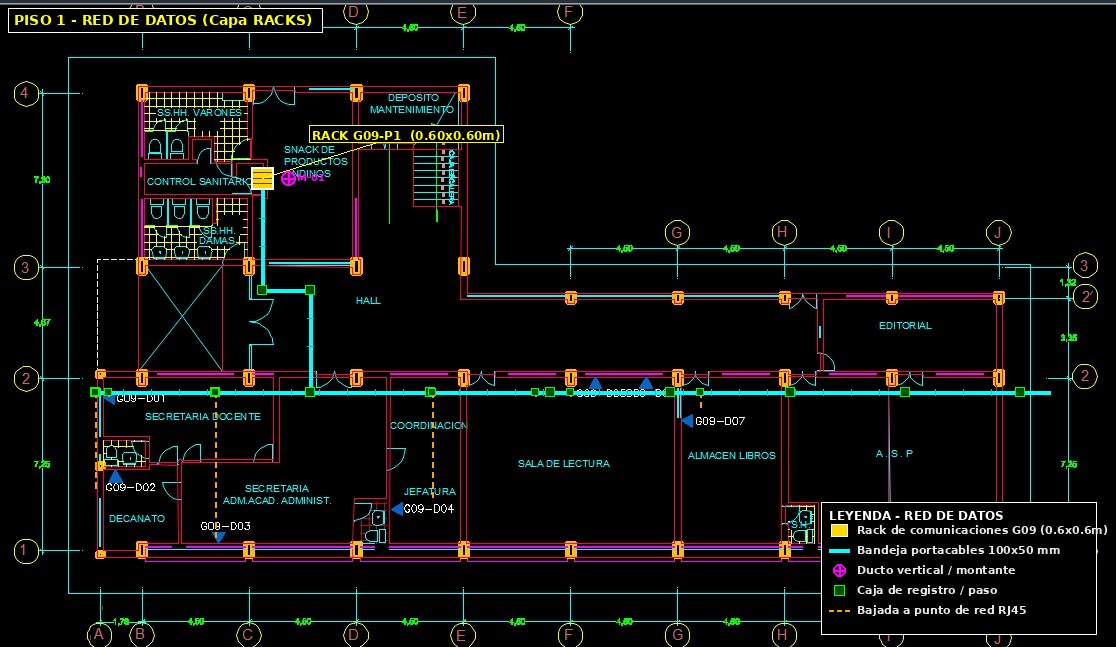
\includegraphics[width=1.0\linewidth]{figures/figuresMarco/primer_nivel.jpeg}
                \caption{}
                \label{fig:placeholder}
            \end{figure}

        \item Piso 2: 6 puntos (D08 a D13)
        
            \begin{figure}[H]
                \centering
                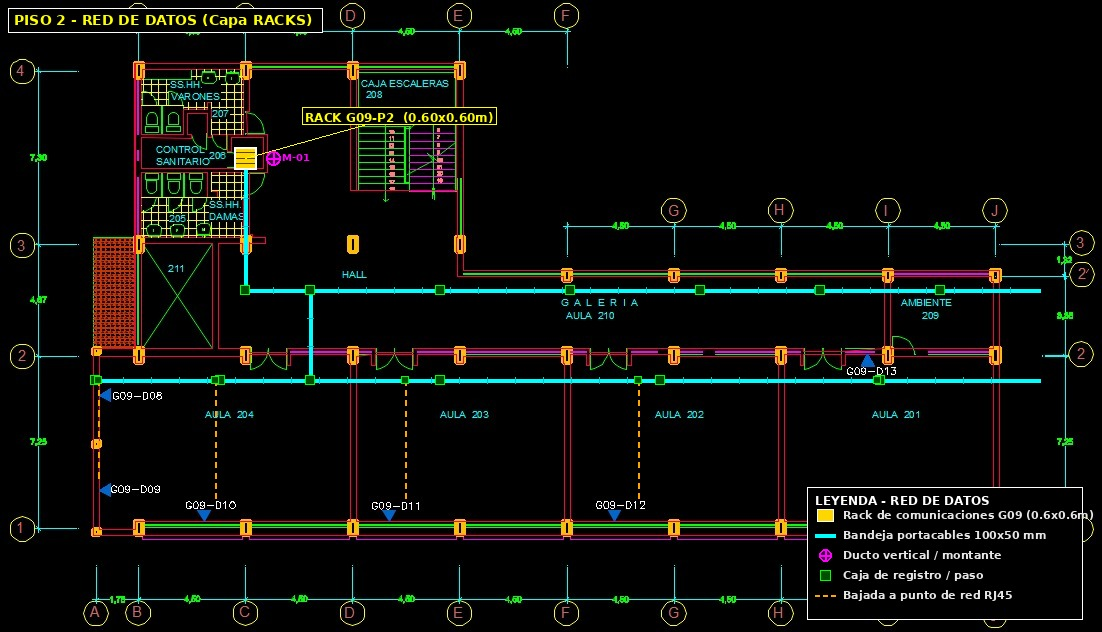
\includegraphics[width=1.0\linewidth]{figures/figuresMarco/segundo_nivel.jpeg}
                \caption{}
                \label{fig:placeholder}
            \end{figure}


        \item Piso 3: 15 puntos (D14 a D29), destacando el laboratorio con 10 puntos concentrados
        
            \begin{figure}[H]
                \centering
                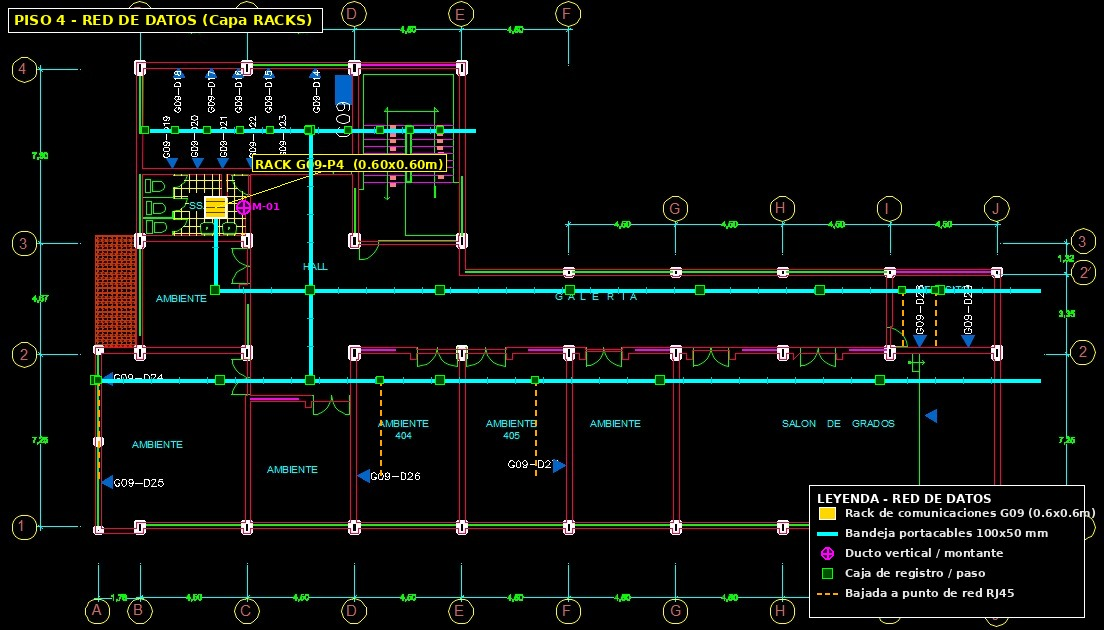
\includegraphics[width=1.0\linewidth]{figures/figuresMarco/tercer_nivel.jpeg}
                \caption{}
                \label{fig:placeholder}
            \end{figure}

    \end{itemize}
    
    \item \textbf{Racks}: Se proyecta \textbf{1 Rack Principal (MDF)} ubicado en el Tercer Nivel (identificado como el bloque azul G09), que centralizará la conexión de todo el edificio
    
    \item \textbf{Cobertura}: 100\% de las oficinas administrativas, aulas teóricas y laboratorios especializados
\end{itemize}

\section{Justificación técnica y beneficios}

\section{Normas y estándares aplicados}

\chapter{Planos}

\section{Plano de ubicación general de la red}

\section{Planos de planta con puntos de red y canalizaciones}

\section{Plano de racks, patch panels y salas de telecomunicaciones}

\section{Plano de backbone}

\section{Detalles constructivos de ductos, bandejas y registros}

Para la implementación física se seguirán las normas \textbf{ANSI/TIA-569-D} :

\begin{itemize}
    \item \textbf{Bandejas portacables}: En los pasillos principales (rutas troncales), se instalarán bandejas tipo escalerilla o bandejas metálicas perforadas de 200x50 mm suspendidas sobre el cielo raso para organizar el backbone y el cableado horizontal.
    
    \item \textbf{Ductería}: Se utilizará \textbf{tubo conduit de PVC de 1 ¼"} para los pases de muros y áreas estratégicas, asegurando un radio de curvatura mínimo para no dañar los cables Cat6A.
    
    \item \textbf{Canaletas}: En interiores de aulas y oficinas, se emplearán canaletas de PVC autoextinguible (tipo 20x12 mm o 40x25 mm) adosadas a la pared para una distribución estética.
    
    \item \textbf{Registros}: Se instalarán cajas de paso de PVC de 150x150x80 mm en cada derivación importante para facilitar el mantenimiento y futuras expansiones.
\end{itemize}

\begin{figure}[H]
    \centering
    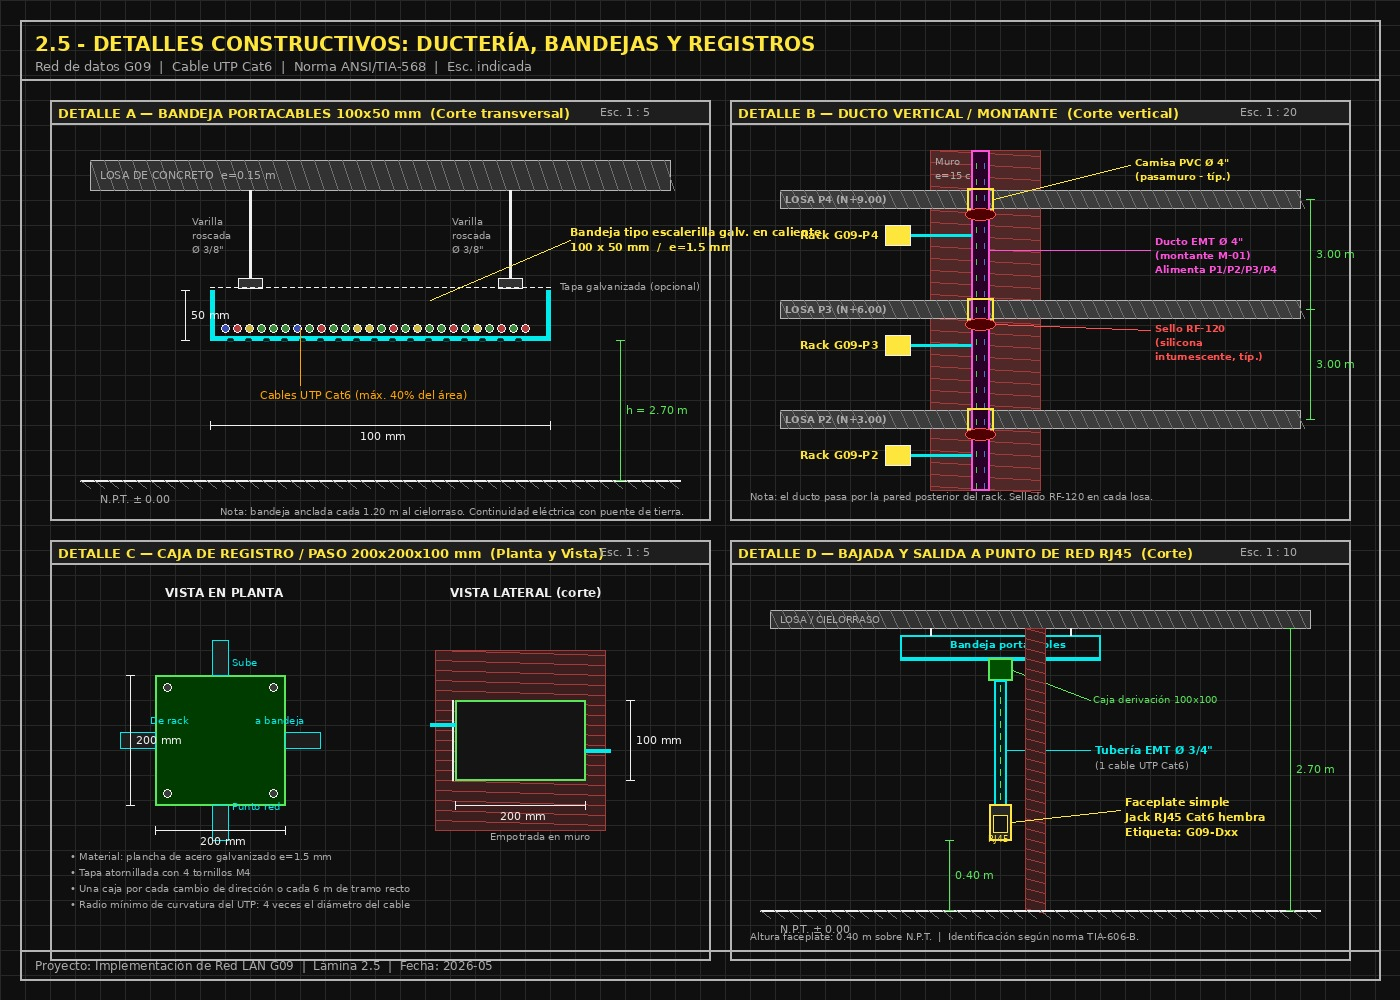
\includegraphics[width=1.0\linewidth]{figures/figuresMarco/detales_constructivos.jpeg}
    \caption{}
    \label{fig:placeholder}
\end{figure}

\section{Diagrama de puesta a tierra}

\chapter{Especificaciones Técnicas}

\section{Tipo y categoría de cables}

\section{Normas de instalación, etiquetado y terminación}

\section{Estándares de racks y gabinetes}

\section{Equipos pasivos y activos}
La infraestructura del sistema de cableado estructurado requiere componentes
activos y pasivos que permitan garantizar conectividad, organización y adecuada
administración de la red.
% -----------------------------------------------------------
\subsection{Equipos pasivos}
% -----------------------------------------------------------
Los equipos pasivos corresponden a los elementos físicos del sistema de
telecomunicaciones que no requieren alimentación eléctrica para su funcionamiento.
% -----------------------------------------------------------
\subsubsection{Cable UTP Categoría 6}
% -----------------------------------------------------------

Se utilizará cable UTP Categoría 6 para el cableado horizontal del edificio,
permitiendo velocidades de transmisión de hasta 1 Gbps y frecuencias de
operación de 250 MHz.

\begin{table}[H]
\centering
\caption{Especificaciones del cable UTP Cat.6}
\begin{tabular}{|c|c|}
\hline
\textbf{Característica} & \textbf{Especificación} \\
\hline
Tipo & UTP Categoría 6 \\
\hline
Ancho de banda & 250 MHz \\
\hline
Velocidad soportada & 1 Gbps \\
\hline
Norma & ANSI/TIA-568-C.2 \\
\hline
\end{tabular}
\end{table}

% -----------------------------------------------------------
\subsubsection{Patch Panels}
% -----------------------------------------------------------

Los patch panels permiten organizar y administrar las terminaciones del cableado
horizontal dentro del rack principal de telecomunicaciones.

\begin{table}[H]
\centering
\caption{Características de los Patch Panels}
\begin{tabular}{|c|c|}
\hline
\textbf{Característica} & \textbf{Especificación} \\
\hline
Tipo & Patch Panel Cat.6 \\
\hline
Capacidad & 24 puertos \\
\hline
Montaje & Rack 19'' \\
\hline
Cantidad proyectada & 3 unidades \\
\hline
\end{tabular}
\end{table}

% -----------------------------------------------------------
\subsubsection{Faceplates y Keystone Jack}
% -----------------------------------------------------------

Los puntos de usuario estarán implementados mediante faceplates dobles con
conectores RJ-45 categoría 6, permitiendo conexión para equipos de datos y voz.

\begin{table}[H]
\centering
\caption{Características de faceplates y keystone jack}
\begin{tabular}{|c|c|}
\hline
\textbf{Elemento} & \textbf{Especificación} \\
\hline
Faceplate & Doble puerto RJ-45 \\
\hline
Keystone Jack & Cat.6 RJ-45 \\
\hline
Compatibilidad & ANSI/TIA-568-C \\
\hline
\end{tabular}
\end{table}

% -----------------------------------------------------------
\subsubsection{Rack de telecomunicaciones}
% -----------------------------------------------------------

El MDF contará con un gabinete metálico de 42U para alojar equipos activos y
pasivos de telecomunicaciones.

\begin{table}[H]
\centering
\caption{Características del rack principal}
\begin{tabular}{|c|c|}
\hline
\textbf{Característica} & \textbf{Especificación} \\
\hline
Tipo & Rack cerrado 19'' \\
\hline
Altura & 42U \\
\hline
Ancho & 600 mm \\
\hline
Profundidad & 800 mm \\
\hline
Ventilación & Ventiladores internos \\
\hline
\end{tabular}
\end{table}

% -----------------------------------------------------------
\subsection{Equipos activos}
% -----------------------------------------------------------

Los equipos activos son dispositivos electrónicos encargados de procesar,
administrar y distribuir el tráfico de red dentro de la infraestructura de
telecomunicaciones.

% -----------------------------------------------------------
\subsubsection{Switch de distribución}
% -----------------------------------------------------------

El MDF contará con un switch administrable Gigabit Ethernet encargado de la
distribución principal de la red del edificio.

\begin{table}[H]
\centering
\caption{Características del switch de distribución}
\begin{tabular}{|c|c|}
\hline
\textbf{Característica} & \textbf{Especificación} \\
\hline
Puertos & 24 puertos Gigabit Ethernet \\
\hline
Uplinks & 4 puertos SFP+ \\
\hline
Administración & Layer 2 administrable \\
\hline
Alimentación PoE & Compatible PoE+ \\
\hline
Velocidad & 10/100/1000 Mbps \\
\hline
\end{tabular}
\end{table}

% -----------------------------------------------------------
\subsubsection{Access Points Wi-Fi}
% -----------------------------------------------------------

Se instalarán Access Points Wi-Fi 6 para brindar cobertura inalámbrica en áreas
académicas y administrativas del edificio.

\begin{table}[H]
\centering
\caption{Características de los Access Points}
\begin{tabular}{|c|c|}
\hline
\textbf{Característica} & \textbf{Especificación} \\
\hline
Estándar & IEEE 802.11ax \\
\hline
Bandas & 2.4 GHz y 5 GHz \\
\hline
Tecnología & MU-MIMO y OFDMA \\
\hline
Alimentación & PoE+ \\
\hline
Capacidad & Hasta 500 usuarios \\
\hline
\end{tabular}
\end{table}

% -----------------------------------------------------------
\subsubsection{UPS}
% -----------------------------------------------------------

El rack principal contará con un sistema UPS encargado de proteger los equipos
de telecomunicaciones frente a cortes eléctricos y variaciones de tensión.

\begin{table}[H]
\centering
\caption{Características del UPS}
\begin{tabular}{|c|c|}
\hline
\textbf{Característica} & \textbf{Especificación} \\
\hline
Capacidad & 1500 VA \\
\hline
Autonomía & 30 minutos \\
\hline
Función & Respaldo eléctrico \\
\hline
Tipo & UPS interactiva \\
\hline
\end{tabular}
\end{table}
\section{Requisitos eléctricos y de puesta a tierra}

\section{Procedimientos de certificación}

%\printbibliography
\clearpage
\phantomsection   
\include{bib}

\end{document}
